\section{Operational Design Domain}

As we have already seen, the SAE levels of automation are all about what the vehicle does (lateral and longitudinal control), who supervises the driving task, who drives in the edge cases and \textbf{where the vehicle drives}.
This last point is the \textbf{Operational Design Domain} (ODD), one of the key concepts of autonomous driving.

To deploy a vehicle without a driver we need an extremely high safety integrity level, around \textbf{99.9999\%} (the ``six-nines imperative'').
If the vehicle had to operate \textbf{everywhere}, in an unbounded environment, verifying this level of safety would be \textbf{mathematically impossible}.
The ODD defines the exact envelope inside which the autonomy can be formally proven to be safe.

So, before designing anything, we have to understand \textbf{what} our vehicle has to do and \textbf{where}. The questions are:
\begin{compactitemize}
    \item What is the \textbf{mission} of the vehicle?
    \item What is the \textbf{scenario} where the vehicle drives?
    \item What are the drivers for deciding \textbf{where to mount the sensors}?
\end{compactitemize}

\subsection{Definition}
The ODD is defined by SAE J3016 as the ``\textit{operating conditions under which a given driving automation system or feature thereof is specifically designed to function}''.
There is still no industry-wide standard or guideline at the international level.

Designing the ODD of a vehicle that operates in a specific domain requires a careful consideration of the \textbf{vehicle's capabilities}, of the \textbf{characteristics of its operating environment} and of the \textbf{specific tasks} it will perform.
The ODD is the basis to derive \textbf{requirements} and \textbf{scenarios}: its output can be a set of requirements used to define the functionalities of the autonomous vehicle.

\subsubsection{Formal definition (PAS 1883)}
\noindent\begin{minipage}[c]{0.5\textwidth}
To formally define the ODD we follow the hierarchical taxonomy of the \textbf{PAS 1883} standard, based on three macro domains:
\begin{enumerate}
    \item \textbf{Scenario}: all the physical features that are \textbf{geo-stationary}, such as the drivable area, buildings, landmarks and infrastructure;
    \item \textbf{Environment}: all the elements that surround us, including \textbf{weather}, \textbf{connectivity} and \textbf{time of day};
    \item \textbf{Dynamic elements}: all the \textbf{dynamic actors} of the environment, such as vehicles, people or any other moving machinery.
\end{enumerate}
\end{minipage}\hfill
\begin{minipage}[c]{0.46\textwidth}
    \centering
    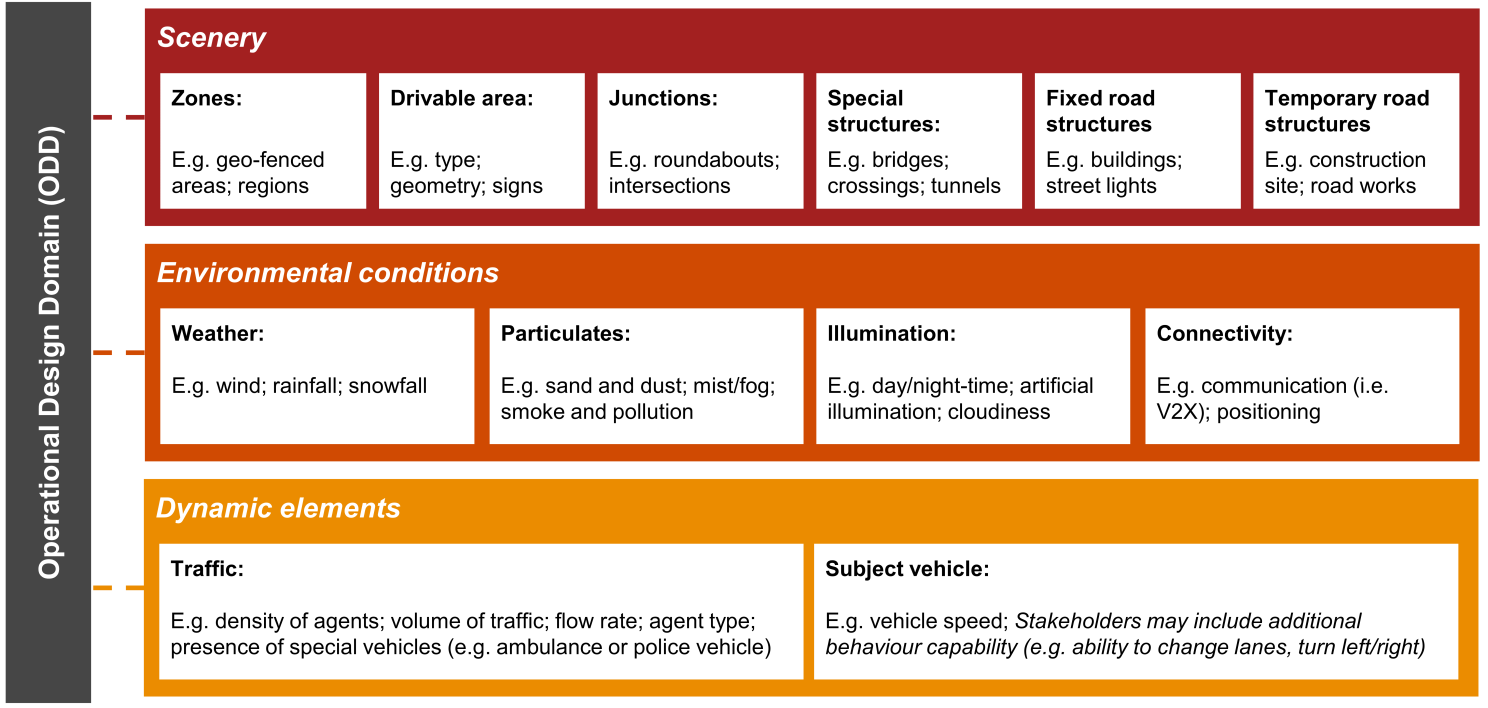
\includegraphics[width=\linewidth]{images/C4_1.png}
    \captionof{figure}{ODD taxonomy (PAS 1883)}
\end{minipage}

\vspace{6pt}In the following tables each domain is applied to an example: an \textbf{autonomous truck} (LGV) operating in a \textbf{port}.

\paragraph{Scenario}
\begin{table}[H]
    \centering
    \small
    \begin{tabular}{|p{2.6cm}|p{6.3cm}|p{6.3cm}|}
        \hline
        \textbf{Aspect} & \textbf{Description} & \textbf{Example} \\
        \hline
        Operating zone & Designated area where the truck is intended to operate within the port & Main terminal area, cargo storage yards, designated driving lanes \\
        \hline
        Operating hazard zone & Areas within the operating zone where the truck's movement can harm people & Loading and unloading zones, pedestrian crossings, areas with heavy equipment \\
        \hline
        Restricted zone & Areas restricted because of hazards or safety concerns & Maintenance areas, zones with low overhead clearance \\
        \hline
        Confined zone & Areas where the movement is restricted due to limited space & Areas with limited manoeuvrability \\
        \hline
        Junctions & Complex intersections or roundabouts the vehicle must navigate safely & Roundabouts connecting terminal areas, junctions near docks \\
        \hline
        Special structures & Structures requiring special attention & Bridges, ramps, tunnels, areas with GPS interference \\
        \hline
    \end{tabular}
    \caption{ODD scenario of an autonomous truck in a port}
\end{table}

\paragraph{Environment}
\begin{table}[H]
    \centering
    \small
    \begin{tabular}{|p{3cm}|p{12.2cm}|}
        \hline
        \textbf{Aspect} & \textbf{Description} \\
        \hline
        Weather conditions & Atmospheric conditions that can affect the operation: temperature, precipitation, wind, fog and snow \\
        \hline
        Particulates & Presence of fine particles, dust, dirt or debris \\
        \hline
        Illumination & Lighting conditions under which the system operates (daylight and night-time) \\
        \hline
        Connectivity & Capability of the system to handle temporary network outages \\
        \hline
    \end{tabular}
    \caption{ODD environment}
\end{table}

\paragraph{Dynamic elements}
The dynamic elements include both the capabilities of the ego vehicle and the traffic around it.

\begin{table}[H]
    \centering
    \small
    \begin{tabular}{|p{2.6cm}|p{5.8cm}|p{6.8cm}|}
        \hline
        \textbf{Aspect} & \textbf{Description} & \textbf{Example requirement} \\
        \hline
        Maximum speed & Maximum speed of the LGV in the port & 20\,km/h \\
        \hline
        Acceleration & Acceleration capabilities & Reach the maximum speed from standstill within 5\,s \\
        \hline
        Braking & How quickly it stops from the maximum speed & Complete stop within 5\,m \\
        \hline
        Load capacity & Maximum weight the LGV can handle & 30 tons \\
        \hline
        Battery life & Battery requirements & At least 8 hours of continuous operation \\
        \hline
        Communication & How it communicates with other vehicles/systems in the port & Wireless communication, e.g.\ WiFi or Bluetooth \\
        \hline
        Obstacle detection & Sensors used to detect obstacles & Combination of sensors, such as LiDAR and cameras \\
        \hline
    \end{tabular}
    \caption{ODD dynamic elements: the ego vehicle}
\end{table}

\begin{table}[H]
    \centering
    \small
    \begin{tabular}{|p{3cm}|p{12.2cm}|}
        \hline
        \textbf{Traffic factor} & \textbf{Description} \\
        \hline
        Density of agents & Number of vehicles or objects in an area of the port: autonomous and regular vehicles, but also workers \\
        \hline
        Volume of traffic & Amount of vehicles entering, exiting and circulating in the designated areas \\
        \hline
        Flow rate & Vehicles passing through a point per unit of time; indicates how efficiently the traffic moves \\
        \hline
        Agent type & Types of vehicles or objects: autonomous, regular and special vehicles \\
        \hline
        Special vehicles & Vehicles not part of the regular traffic flow, such as forklifts, cranes or other heavy machinery \\
        \hline
        Human factors & Interaction with human operators and workers: communication protocols, emergency procedures, ability to respond to human intervention \\
        \hline
    \end{tabular}
    \caption{ODD dynamic elements: traffic}
\end{table}

\subsection{Impact of ODD on sensor positioning}
From the ODD we can derive the requirements of the system, and also understand \textbf{where to install the sensors}.
Different sensor requirements may arise from the ODD definition:
\begin{compactitemize}
    \item \textbf{Field of view}: the placement adapts to the road type (e.g.\ 360° for urban areas, long-range forward for highways);
    \item \textbf{Height and terrain}: the mounting depends on the terrain (e.g.\ high for off-road, low for parking);
    \item \textbf{Obstacle detection}: the ODD defines the required detection range (long-range sensors for high speeds, close-range for low-speed environments);
    \item \textbf{Environmental factors}: sensors are chosen and positioned to mitigate weather and lighting (e.g.\ radar for fog, cameras for clear conditions);
    \item \textbf{Speed}: high speeds require forward-facing sensors with high frequency and range, while low speeds need a comprehensive side and rear coverage.
\end{compactitemize}

\subsubsection{Example: AGV sensor setup}
\noindent\begin{minipage}[c]{0.6\textwidth}
A good example is an AGV (Automated Guided Vehicle) operating in a container port, whose sensor setup is derived directly from its ODD:
\begin{enumerate}
    \item an \textbf{elevated roof mast} with a 360° LiDAR, for SLAM localization in the container alleys, where GNSS is not available;
    \item a \textbf{front 77\,GHz radar}, for Doppler velocity tracking and emergency braking within 5\,m even in dense fog;
    \item \textbf{four corner LiDARs and short-range radars}, for hazard protection down to ground level and in blind turns (ISO 3691-4);
    \item a \textbf{lateral proximity array}, to monitor the side clearance in the confined container slots.
\end{enumerate}
\end{minipage}\hfill
\begin{minipage}[c]{0.36\textwidth}
    \centering
    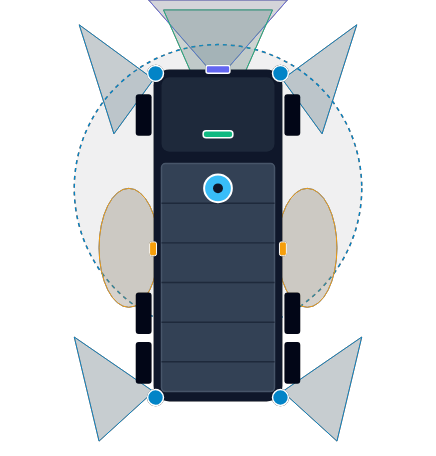
\includegraphics[width=0.8\linewidth]{images/C4_2.png}
    \captionof{figure}{AGV sensor setup}
\end{minipage}

\subsection{Sensor configuration design}
\noindent\begin{minipage}[c]{0.6\textwidth}
Sensor positioning is what enables the vehicle to perceive its surroundings.
Different functionalities and requirements must be guaranteed, using sensors with different precision and characteristics; redundancy and reliability are important, and of course there is always a \textbf{budget}.

\vspace{4pt}Again, the ODD must be considered when designing the sensor setup: for lane keeping on a highway, one radar in front of the car should be enough, while for AD in urban environments a \textbf{360° horizontal coverage} with all three major modalities (camera, LiDAR and radar) is required to reliably detect the traffic.
\end{minipage}\hfill
\begin{minipage}[c]{0.36\textwidth}
    \centering
    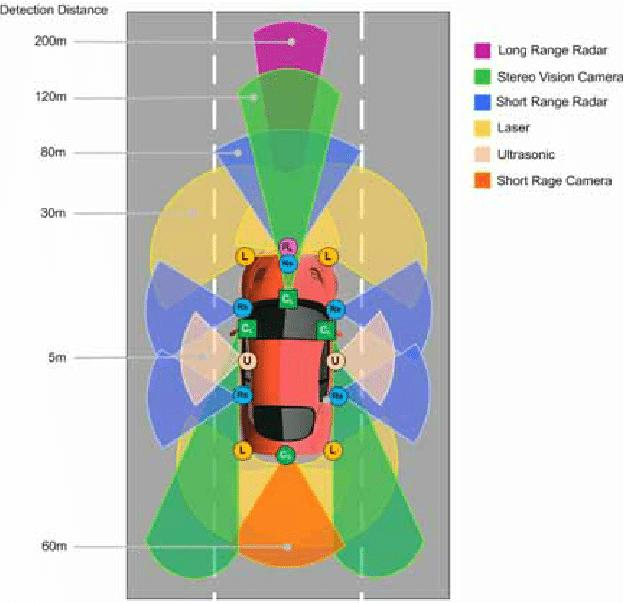
\includegraphics[width=\linewidth]{images/C4_3.png}
    \captionof{figure}{Coverage of the sensors of an urban AD vehicle}
\end{minipage}

\vspace{6pt}In the following figures, the blue/green/yellow areas are the sensor coverage and the red areas are the \textbf{blind spots}.

\subsubsection{LiDAR}
There are several possible configurations for the LiDARs:
\begin{compactitemize}
    \item \textbf{LiDAR on the roof center}: a simple setup, with 360° coverage from one sensor and no effort to synchronize and align multiple point clouds. However, it has \textbf{many blind spots} around the vehicle (localization/detection).
    \item \textbf{Multiple tilted LiDARs on the roof}: the best coverage among the roof-mounted configurations, but a higher complexity in terms of integration and point cloud fusion (mapping/navigation).
    \item \textbf{Front LiDAR}: a good and simple solution to detect the vehicles in front, but it does not work well on \textbf{slopes} (detection); a solid-state LiDAR can be used.
    \item \textbf{Side-view LiDARs}: full coverage of the sides of the vehicle but, again, they do not work well on slopes (solid-state LiDARs).
\end{compactitemize}

\begin{figure}[H]
    \centering
    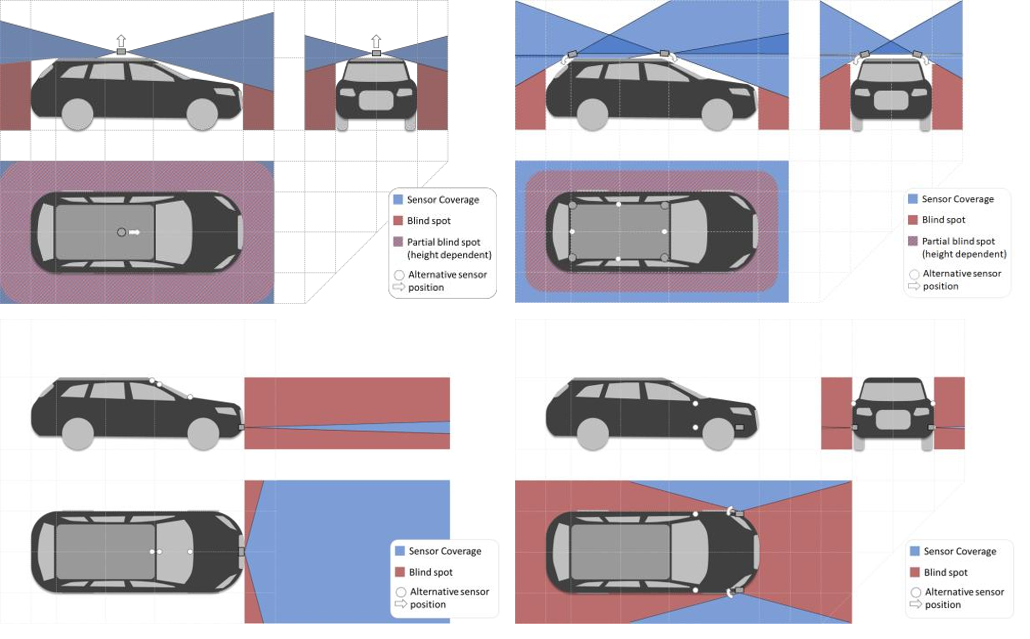
\includegraphics[width=0.75\textwidth]{images/C4_4.png}
    \caption{LiDAR configurations: roof center, tilted roof LiDARs, front and side-view}
\end{figure}

\subsubsection{Radar}
Radars are usually mounted in the lower part of the vehicle, on the sides and in the corners.
A \textbf{360° coverage} with short- and mid-range radars gives a good coverage of the environment, but their vertical FoV is a challenge on non-flat terrain (safety, collision warning).
A \textbf{front radar}, mid-range (MRR, $\sim$100\,m) or long-range (LRR, $\sim$250\,m), enables ADAS features like adaptive cruise control (ACC) and autonomous emergency braking (AEB), but alone it is not sufficient for urban AD.

\begin{figure}[H]
    \centering
    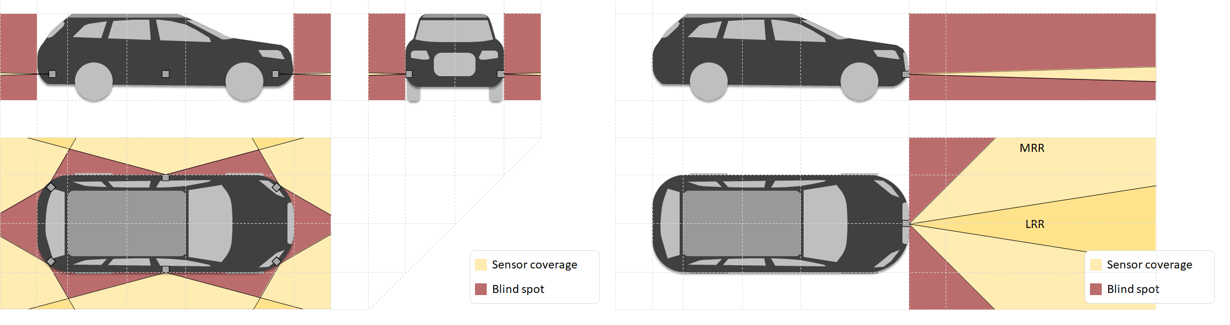
\includegraphics[width=0.75\textwidth]{images/C4_5.png}
    \caption{360° radar coverage and front radar}
\end{figure}

\subsubsection{Camera}
The typical camera configurations are:
\begin{compactitemize}
    \item \textbf{360° coverage with roof-mounted wide-angle cameras}: it allows to build a bird's-eye view of the environment (mapping and/or localization);
    \item \textbf{Central camera tower}: used for mapping (feature extraction);
    \item \textbf{Front camera}: mounted on the windshield, it enables ADAS features like lane keeping, lane departure warning or lane change assist. Its vertical FoV is limited by the hood (object detection);
    \item \textbf{Wide-angle camera for traffic light detection}: an alternative configuration mounted on the roof.
\end{compactitemize}

\begin{figure}[H]
    \centering
    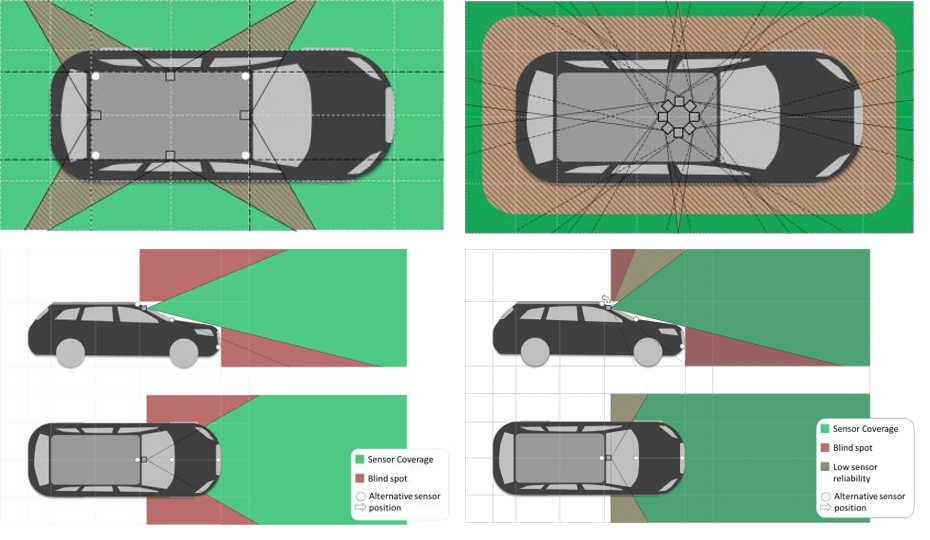
\includegraphics[width=0.65\textwidth]{images/C4_6.png}
    \caption{Camera configurations}
\end{figure}

\paragraph{Camera mounting issues}
Where we place the cameras (and in general the sensors) also creates some problems:
\begin{compactitemize}
    \item \textbf{Mid-air and ceiling obstacles}: open truck doors, protruding freight, tree branches, boom gates or low bridges may not be seen by sensors mounted too low;
    \item \textbf{Slopes}: where a climb starts, the ramp in front of the vehicle can be interpreted as an obstacle;
    \item \textbf{Cyclists}: sensors mounted high on the roof may have blind spots close to the vehicle, e.g.\ they may not detect a cyclist on the side;
    \item \textbf{Crossings with occlusions}: a sensor facing sideways can help.
\end{compactitemize}

\begin{figure}[H]
    \centering
    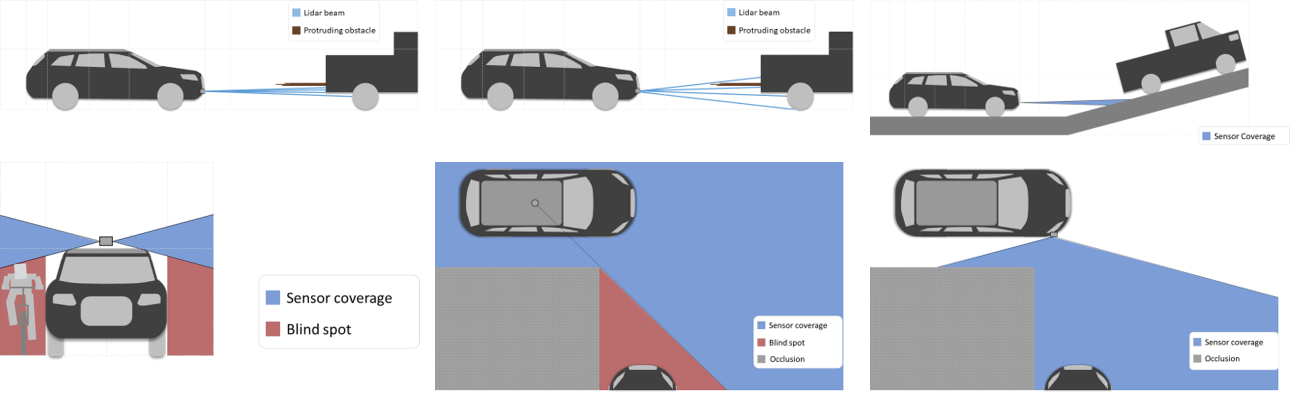
\includegraphics[width=0.75\textwidth]{images/C4_7.png}
    \caption{Mounting issues: protruding obstacles, slopes, cyclists and occlusions}
\end{figure}

\subsection{Exercise: last-mile delivery robot}
In class we tried to define the ODD and the sensor suite of a \textbf{last-mile delivery vehicle} (e.g.\ for deliveries in Modena).
The answer depends completely on the ODD, as the two classes of real products show:

\begin{figure}[H]
    \centering
    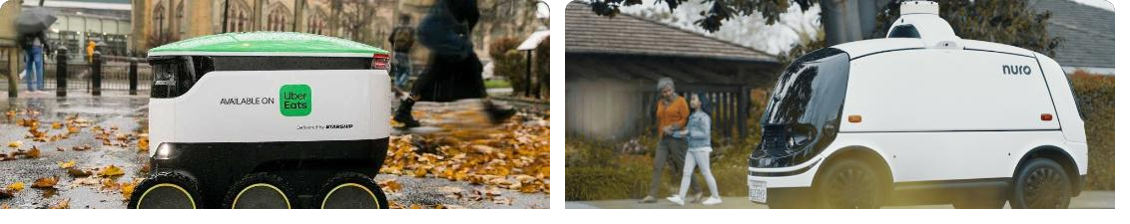
\includegraphics[width=0.75\textwidth]{images/C4_8.png}
    \caption{Sidewalk micro-bot (left) and on-road pod (right)}
\end{figure}

\begin{table}[H]
    \centering
    \small
    \begin{tabular}{|p{2.4cm}|p{6.3cm}|p{6.3cm}|}
        \hline
         & \textbf{Sidewalk micro-bot (Starship class)} & \textbf{On-road pod (Nuro R2/R3 class)} \\
        \hline
        \textbf{ODD} & Pedestrian walkways and campuses, $\leq$ 6\,km/h & Public neighbourhood streets, $\leq$ 45--72\,km/h \\
        \hline
        \textbf{Sensors} & Vision-centric: 12 surround cameras + stereo pairs; ultrasonic array for low curb edges & Elevated top tower with 360° LiDAR + 360° HDR cameras; front and corner 77\,GHz radars for all weather \\
        \hline
        \textbf{Safety} & Low kinetic risk: the 6\,km/h cap avoids a heavy roof LiDAR & Automotive scale: external airbags for pedestrians \\
        \hline
    \end{tabular}
    \caption{Two last-mile delivery ODDs}
\end{table}

\begin{infobox}[Why small robots can use only cameras]
The small sidewalk robots can rely only on cameras, without LiDAR: since they move slowly, even if the cameras have a non-negligible error (e.g.\ in depth estimation), it is not a big problem.
The same small error becomes important at high speeds, which is why on-road vehicles need LiDAR and radar.
\end{infobox}

\subsection{Conclusions}
\begin{compactitemize}
    \item \textbf{Safety contract}: the ODD formally bounds the operational envelope, so that safety can be proven;
    \item \textbf{Blind spot geometry}: chassis height and pitch dynamics require low perimeter sensor pods;
    \item \textbf{Cross-modal triad}: LiDAR for geometry, (4D) radar for weather, cameras for semantics;
    \item \textbf{Bespoke topology}: a sensor suite is the exact projection of the specific operational risks.
\end{compactitemize}
The takeaway: \textbf{never design a sensor suite in the abstract}, always derive it from the ODD boundaries.
